\documentclass[UTF8,12pt,a4paper]{ctexart}

\usepackage{amsmath,amssymb,bm}
\usepackage{array,booktabs,tabularx,longtable}
\usepackage{geometry}
\usepackage{graphicx}
\usepackage{float}
\usepackage{xcolor}
\usepackage{enumitem}
\usepackage{siunitx}
\usepackage{hyperref}

\geometry{left=2.45cm,right=2.45cm,top=2.35cm,bottom=2.35cm}
\graphicspath{{../figures/}}
\hypersetup{colorlinks=true,linkcolor=blue,urlcolor=blue}
\setlength{\parindent}{2em}
\setlength{\parskip}{0.35em}
\setlength{\emergencystretch}{3em}
\renewcommand{\arraystretch}{1.18}

\title{2025 年高教社杯全国大学生数学建模竞赛 B 题\\[0.4em]
问题三：多光束干涉影响及厚度修正}
\author{独立求解与可复现数值实现}
\date{}

\begin{document}
\maketitle

\begin{abstract}
问题三要求讨论薄膜内部多次往返反射产生多光束干涉的必要条件及其对厚度
测量精度的影响，并判断附件 3、4 的硅（Si）光谱是否存在该现象；若附件
1、2 的碳化硅（SiC）光谱也存在多光束干涉，则需要消除其影响并给出修正结果。
本文从空气--外延层--衬底的 Fresnel 振幅叠加出发，将问题一中的双光束模型
推广为可控的 Airy 几何级数模型。首先用波数域 FFT 和光谱峰间距确定稳定的
硅拟合波段及厚度初值；随后在两个入射角之间共享厚度和材料参数，分别比较
双光束、完全相干多光束和带有效相干系数的部分多光束模型。最终硅数据选择的
部分多光束拟合给出
\[
\boxed{d_{\mathrm{Si}}=3.390020843\ \mu\mathrm{m}},
\qquad \boxed{\eta=0.711511282},
\]
相对于双光束模型的 BIC 改善量为 $247.882121$，说明附件 3、4 中高阶往返
不能简单忽略。对 SiC 附件 1、2 采用精确相干 Airy 模型重新拟合后得到
\[
\boxed{d_{\mathrm{SiC}}^{(3)}=7.399475918\ \mu\mathrm{m}},
\]
相比问题二双光束结果 $7.400452153\ \mu\mathrm{m}$ 仅变化
$-0.000976235\ \mu\mathrm{m}$，相对变化约 $-0.0132\%$。因此，Si 的多光束
效应是本问的主要可观测对象；SiC 中高阶往返的修正虽已完成，但对最终厚度的
数值影响很小。
\end{abstract}

\section{题面约束、任务边界与符号}

为避免把题面给出的信息、用户要求和本次计算中的建模假设混在一起，三者
分别列出如下。

\begin{description}[leftmargin=5em]
  \item[题面事实]
  题面给出了四个 Excel 光谱附件：附件 1、2 对应 SiC，入射角分别为
  $10^\circ$ 和 $15^\circ$；附件 3、4 对应 Si，入射角分别为 $10^\circ$
  和 $15^\circ$。每个附件的第一列是波数 $\sigma$，单位为
  $\mathrm{cm}^{-1}$，第二列是反射率，单位为百分数。问题三要求给出多光束
  干涉的必要条件，分析其对厚度精度的影响，处理附件 3、4，并在必要时修正
  附件 1、2 的结果。
  \item[本次用户任务]
  只完成问题三，结果必须保存在
  \verb|F:/数学建模/2025B/题目3_完整交付| 的独立目录中，同时提供完整
  LaTeX、可运行代码、图表、原始附件副本、数值结果和编译后的 PDF；既有的
  问题一、问题二文件不覆盖、不改写。
  \item[本节额外假设]
  题面附件只提供反射率曲线，没有逐波数给出完整复折射率。因此，为使全谱
  反演可计算，硅的无载流子背景折射率采用代码中明确记录的 Sellmeier 关系，
  并为外延层和衬底各引入一个无损 Drude 代理参数。仪器的幅值归一化和基线
  差异用每个角度一个有界线性校准项吸收。这些是模型假设或 nuisance 参数，
  不是从附件直接测得的材料常数。
\end{description}

本文使用的主要符号为：$d$ 为外延层厚度，$n_0,n_1,n_2$ 分别为空气、外延
层和衬底的复折射率，$\theta_0,\theta_1$ 分别为入射角和层内折射角，$r_{ij}$、
$t_{ij}$ 为从介质 $i$ 到介质 $j$ 的 Fresnel 振幅系数，$\eta$ 为高阶返回的
有效保留系数，$R$ 为反射率。

\section{多光束干涉的物理条件与精度影响}

\subsection{相邻光束的相位关系}

考虑空气--外延层--衬底三层结构。第一束反射光在空气--外延层界面直接反射；
第二束光进入外延层，在外延层--衬底界面反射后从上表面透射出来；后续光束
则在外延层内继续往返。由 Snell 定律
\[
n_0\sin\theta_0=n_1\sin\theta_1,
\]
相邻两束出射光的几何光程差为
\[
\Delta L=2n_1d\cos\theta_1.
\]
用波数 $\sigma=1/\lambda$ 表示时，相位差为
\begin{equation}
  \Delta\phi=2\pi\sigma\Delta L
  =4\pi\sigma n_1d\cos\theta_1,
  \label{eq:phase}
\end{equation}
其中在程序中 $\sigma$ 以 $\mathrm{cm}^{-1}$ 输入，而 $d$ 先由微米换算为
厘米。式 \eqref{eq:phase} 是所有后续光束叠加和厚度反演的核心。

\subsection{多光束的必要条件}

多光束效应不是“只要是薄膜就必然存在”。它至少需要下列条件同时具备：

\begin{enumerate}[label=(\arabic*)]
  \item \textbf{时间相干或等效相干：} 光源在相邻往返的时间差内保持足够相干，
  或仪器的窄带分辨率使各次返回在测量中仍可相干叠加；否则不同返回的交叉项
  在时间或频率平均后消失。
  \item \textbf{高阶返回具有非零振幅：} 设一次高阶返回相对于前一次的振幅比
  的模为
  \begin{equation}
    \rho(\sigma)=\left|r_{10}(\sigma)r_{12}(\sigma)
    \exp\left(i\Delta\phi(\sigma)\right)\right|.
    \label{eq:rho}
  \end{equation}
  只要 $\rho$ 很小，第二次及以后的返回会迅速衰减，多光束虽物理上存在，
  但对反射率的可观测影响可能小于噪声；当 $\rho$ 达到百分之几到百分之十量级
  时，高阶项就可能改变条纹的对比度和相位。
  \item \textbf{相位变化可分辨：} 测量波数分辨率、采样步长和有效光谱范围应能
  解析 $\Delta\phi$ 随 $\sigma$ 的变化。若一条光谱内只包含很少条纹，或条纹
  被仪器线宽、采样和后处理平滑掉，则难以从数据识别多光束项。
  \item \textbf{角度和空间平均不能完全洗掉条纹：} 光束发散、探测器数值孔径、
  表面粗糙度或厚度横向不均匀会导致不同角度、不同位置的相位平均。如果这种
  平均足够强，多光束的相干特征会被压低。
\end{enumerate}

上述条件是必要条件而非充分条件。特别是 $\rho>0$ 只能说明存在高阶返回，
不保证一定能在有限噪声的实验曲线上显著识别；最终仍需用嵌套模型比较、残差
和角度一致性进行数据层面的判断。

\subsection{从双光束到 Airy 几何级数}

对偏振 $q\in\{s,p\}$，问题一的双光束振幅可写成
\begin{equation}
  A_q^{(0)}=r_{01,q}+t_{01,q}r_{12,q}t_{10,q}
  \exp(i\Delta\phi).
  \label{eq:two-beam}
\end{equation}
第二项是第一次进入薄膜并在下界面反射后返回的光。若继续保留后续
往返，每增加一次在薄膜中的循环，就多乘一个
\begin{equation}
  z_q=r_{10,q}r_{12,q}\exp(i\Delta\phi).
  \label{eq:z}
\end{equation}
因此相干叠加为
\begin{align}
  A_q^{(\infty)}
  &=r_{01,q}+t_{01,q}r_{12,q}t_{10,q}
    \exp(i\Delta\phi)\sum_{m=0}^{\infty}z_q^m \\ 
  &=r_{01,q}+\frac{t_{01,q}r_{12,q}t_{10,q}
    \exp(i\Delta\phi)}{1-r_{10,q}r_{12,q}\exp(i\Delta\phi)}.
  \label{eq:airy}
\end{align}
当 $|z_q|<1$ 时，几何级数收敛。代码没有用截断的若干项近似，而是直接使用
式 \eqref{eq:airy}，从而避免在高反射区因截断阶数不同而产生额外误差。

为了把“完全相干”和“实验中存在部分平均”区分开，本文还使用一个诊断模型
\begin{equation}
  A_q(\eta)=r_{01,q}+\frac{t_{01,q}r_{12,q}t_{10,q}
  \exp(i\Delta\phi)}{1-\eta r_{10,q}r_{12,q}\exp(i\Delta\phi)},
  \qquad 0\leq\eta\leq1.
  \label{eq:partial}
\end{equation}
其中 $\eta=0$ 恢复双光束式 \eqref{eq:two-beam}，$\eta=1$ 恢复精确相干
Airy 式 \eqref{eq:airy}。中间值不是直接测得的“相干长度”，而是衡量数据
中高阶返回有效程度的部分相干代理参数。非偏振反射率取两个偏振强度的算术
平均：
\begin{equation}
  R(\sigma)=\frac{1}{2}\left(|A_s(\eta)|^2+|A_p(\eta)|^2\right),
  \qquad R_{\%}=100R.
  \label{eq:unpolarized}
\end{equation}

\subsection{为什么忽略多光束会影响厚度}

双光束模型只保留 $m=0$ 项。高阶项不仅改变反射率的幅值，还通过分母
$(1-\eta z_q)^{-1}$ 改变条纹极值位置附近的相位响应。若仍用双光束模型拟合，
优化器可能通过改变 $d$、折射率或幅值校准来补偿这部分结构，于是得到的是
“把多光束误差投影到厚度参数上”的结果。其影响有三种表现：

\begin{itemize}
  \item 条纹对比度的系统偏差，使拟合残差在峰谷附近呈有规律的正负交替；
  \item 不同入射角对 $\cos\theta_1$ 的响应不同，错误模型可能在两个角度给出不
  完全一致的厚度；
  \item 在高反射或界面反射较强的波数段，厚度的局部灵敏度会被高阶相位项
  改写，导致模型选择造成的系统误差超过随机噪声。
\end{itemize}

因此，本文不把“峰间距初值相近”作为多光束是否存在的判据，而是将双光束和
多光束模型放在同一数据、同一校准边界、同一优化流程下进行嵌套比较。

\section{数据读取、完整性审计与拟合波段}

\subsection{原始附件审计}

代码从独立目录下的 \verb|data/附件1.xlsx| 至 \verb|data/附件4.xlsx| 读取
第一个工作表前两列。原始 Excel 只读不改。四个文件均有 7469 行数值数据，
波数升序、无重复值，采样步长中位数为 $0.482\ \mathrm{cm}^{-1}$。每个文件
第一行反射率都恰为 $0\%$，与其后光谱的连续性不一致，所以只在内存中的拟合
数组删除该一个端点，形成 7468 行拟合数据；清洗后的 CSV 同步保存，便于复核。

\begin{table}[H]
  \centering
  \caption{四个附件的输入审计结果}
  \label{tab:audit}
  \small
  \setlength{\tabcolsep}{3pt}
  \begin{tabular}{ccccccc}
    \toprule
    附件 & 材料 & 角度 & 原始行数 & 拟合行数 & 反射率范围(\%) & $>100\%$行数\\
    \midrule
    1 & SiC & $10^\circ$ & 7469 & 7468 & $0\sim95.38499492$ & 0\\
    2 & SiC & $15^\circ$ & 7469 & 7468 & $0\sim102.73935520$ & 262\\
    3 & Si  & $10^\circ$ & 7469 & 7468 & $0\sim79.80197440$ & 0\\
    4 & Si  & $15^\circ$ & 7469 & 7468 & $0\sim91.48944351$ & 0\\
    \bottomrule
  \end{tabular}
\end{table}

附件 2 在局部波数段出现反射率超过 $100\%$ 的记录，这不符合理想反射率的
物理范围，但不能据此擅自截断、重标定或删除数据；本次 SiC 修正仍按题面
提供的原始序列拟合，只用每个角度的有界 affine 校准吸收整体测量比例和基线
差异。四个原始工作簿的 SHA-256 以及审计字段均写在
\verb|results/data_audit.json| 中。

\subsection{硅的背景折射率与有效波段}

硅的背景折射率采用 Sellmeier 形式
\begin{equation}
  n_{\mathrm{Si},0}^2(\lambda)=1+\sum_{j=1}^{3}
  \frac{B_j\lambda^2}{\lambda^2-C_j},
  \qquad \lambda=\frac{10^4}{\sigma}\ (\mu\mathrm{m}),
  \label{eq:sellmeier}
\end{equation}
其中代码中使用
\[
\begin{aligned}
\bm B&=(10.6684293,\ 0.0030434748,\ 1.54133408),\\
\bm C&=(0.0909121907,\ 1.287660172,\ 1218816.0).
\end{aligned}
\]
该关系在本实现中只允许用于 $1.357\sim11.04\ \mu\mathrm{m}$，对应约
$905\sim7369\ \mathrm{cm}^{-1}$。为了避免把有效范围边界附近的外推误差带入
厚度拟合，本文在共同的透明候选区 $1000\sim3600\ \mathrm{cm}^{-1}$ 内比较
波段。

在候选波段 $[L,L+1400]\ \mathrm{cm}^{-1}$ 内，对两个角度分别去除平滑趋势，
计算残差的 FFT 主峰波数间隔，得到粗厚度估计 $d_{\mathrm{FFT}}$。用两个角度
的峰显著性和相对差异构造选择分数
\begin{equation}
  S(L)=\min\{Q_{10}(L),Q_{15}(L)\}
  \left[1-\frac{|d_{10}^{\mathrm{FFT}}-d_{15}^{\mathrm{FFT}}|}
  {\bar d_{\mathrm{FFT}}}\right],
  \label{eq:band-score}
\end{equation}
其中 $Q$ 是 FFT 主峰与谱内中位峰高的比值。该分数只用于选择较稳定的拟合
区间，不直接作为最终厚度。

\begin{table}[H]
  \centering
  \caption{硅候选波段的双角度 FFT 稳定性比较}
  \label{tab:band}
  \small
  \setlength{\tabcolsep}{4pt}
  \begin{tabular}{ccccc}
    \toprule
    候选波段 $(\mathrm{cm}^{-1})$ & $d_{10}^{\mathrm{FFT}}(\mu\mathrm{m})$
    & $d_{15}^{\mathrm{FFT}}(\mu\mathrm{m})$ & 相对差异 & $S(L)$\\
    \midrule
    $1000\sim2400$ & 3.128731 & 3.133654 & 0.1572\% & 1.976614\\
    $1200\sim2600$ & 3.126972 & 3.131884 & 0.1569\% & 2.731156\\
    $1400\sim2800$ & 3.122743 & 3.127638 & 0.1566\% & 2.889118\\
    $1600\sim3000$ & 3.119272 & 3.124150 & 0.1563\% & 3.131473\\
    $1800\sim3200$ & 3.115486 & 3.120348 & 0.1559\% & 3.214800\\
    $2000\sim3400$ & 3.111380 & 3.116222 & 0.1555\% & 4.376882\\
    \bottomrule
  \end{tabular}
\end{table}

因此选择 $2000\sim3400\ \mathrm{cm}^{-1}$ 作为硅的共同拟合区间，共有
5808 个观测值。图 \ref{fig:input-band} 给出了原始光谱、平滑峰以及最终波段。

\begin{figure}[H]
  \centering
  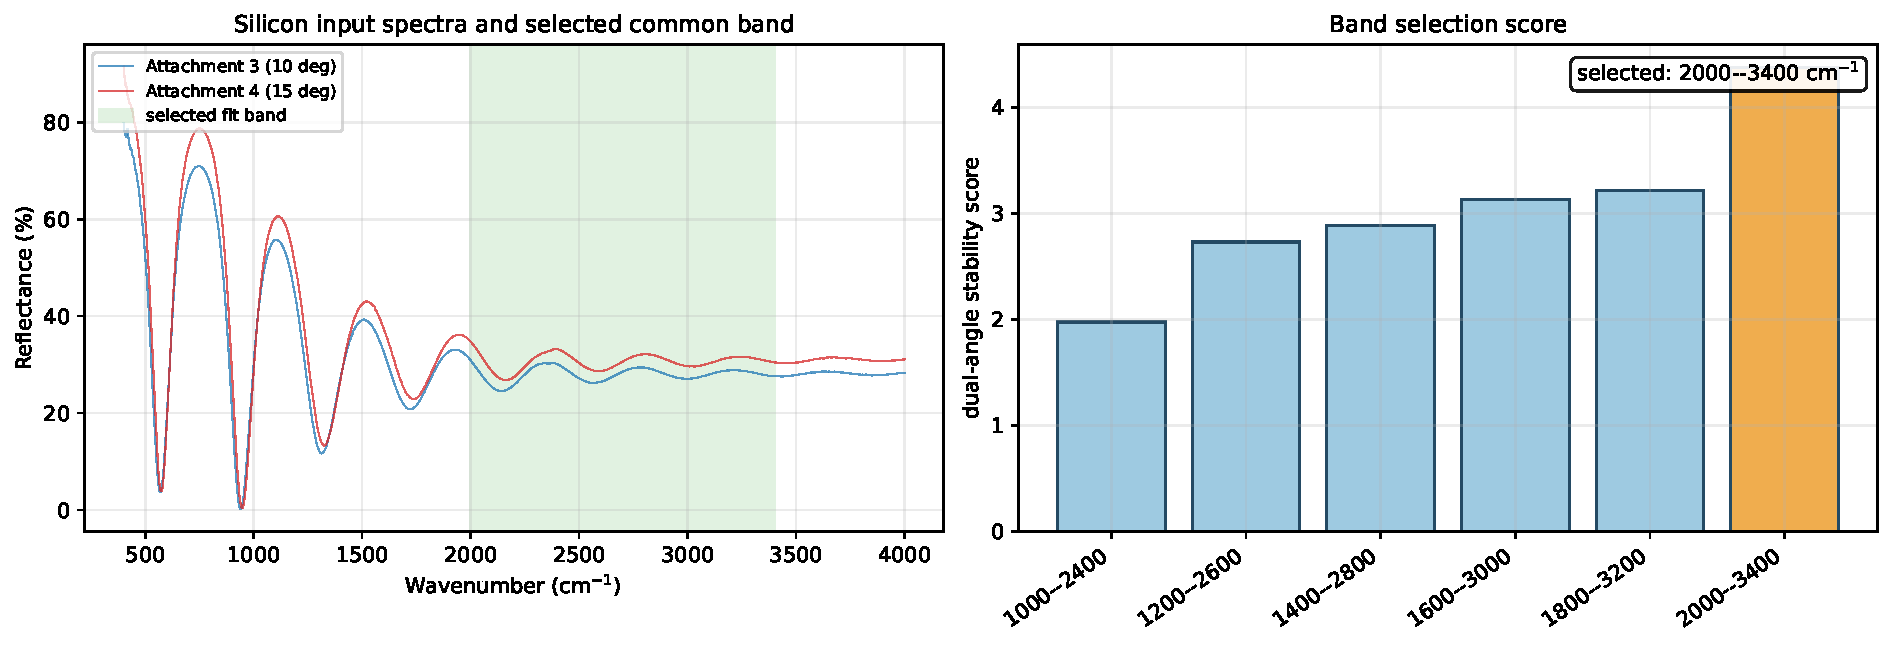
\includegraphics[width=0.98\textwidth]{fig_q3_input_and_band.pdf}
  \caption{附件 3、4 的硅光谱、峰初始化和最终共同拟合波段}
  \label{fig:input-band}
\end{figure}

\subsection{峰间距初始化的作用}

在选定波段内，先用 101 点、三阶多项式的 Savitzky--Golay 滤波器得到平滑
曲线，再搜索显著峰。由相邻峰近似满足 $\Delta\phi=2\pi m$，可用峰间距给出
厚度数量级初值。这一步不把材料色散、偏振和高阶往返完全纳入，所以只用于
初始化和诊断，最终结果必须以全谱反演为准。

\begin{table}[H]
  \centering
  \caption{硅选定波段的峰初始化}
  \label{tab:peaks}
  \small
  \setlength{\tabcolsep}{3.5pt}
  \begin{tabular}{cccccc}
    \toprule
    附件 & 角度 & 检出的峰 $(\mathrm{cm}^{-1})$ & 峰间距中位数
    $(\mathrm{cm}^{-1})$ & $n$ 初值 & $d$ 初值$(\mu\mathrm{m})$\\
    \midrule
    3 & $10^\circ$ & 2380.210, 2782.778, 3207.522 & 413.656 & 3.427453 & 3.531159\\
    4 & $15^\circ$ & 2395.156, 2806.883, 3250.913 & 427.879 & 3.427647 & 3.418968\\
    \bottomrule
  \end{tabular}
\end{table}

两个角度的峰初始化平均值为 $3.475064\ \mu\mathrm{m}$。它与最后的全谱
结果不同并不矛盾：峰间距近似把折射率和条纹阶数视为局部常数，而全谱模型
还同时拟合色散、Fresnel 系数、两个角度的测量校准和多光束分母。

\section{硅的多光束反演模型}

\subsection{色散模型}

为反映透明区中自由载流子代理对层内相位的缓慢影响，代码在 Sellmeier 背景
上使用无损 Drude 修正：
\begin{equation}
  \varepsilon_1(\sigma)=\varepsilon_{\mathrm{Si},0}(\sigma)
  -\frac{\omega_{p,1}^2}{\sigma^2+i\gamma_1\sigma},
  \qquad
  \varepsilon_2(\sigma)=\varepsilon_{\mathrm{Si},0}(\sigma)
  -\frac{\omega_{p,2}^2}{\sigma^2+i\gamma_2\sigma}.
  \label{eq:drude}
\end{equation}
在本次透明带拟合中将 $\gamma_1=\gamma_2=0$，并令
$n_j=\sqrt{\varepsilon_j}$ 取物理支。参数
$(\omega_{p,1},\omega_{p,2})$ 是用于弥补未给出复折射率曲线的模型代理，
不解释为已由附件独立识别的真实等离子体频率。

Fresnel 系数由代码按复 Snell 定律逐点计算。以入射介质 $i$ 和透射介质 $j$
为例，令 $c_i=\cos\theta_i$、$c_j=\cos\theta_j$，则
\begin{align}
 r_s&=\frac{n_ic_i-n_jc_j}{n_ic_i+n_jc_j},
 &t_s&=\frac{2n_ic_i}{n_ic_i+n_jc_j},\\
 r_p&=\frac{n_jc_i-n_ic_j}{n_jc_i+n_ic_j},
 &t_p&=\frac{2n_ic_i}{n_jc_i+n_ic_j}.
 \label{eq:fresnel}
\end{align}
然后将式 \eqref{eq:partial} 代入式 \eqref{eq:unpolarized}，得到每个角度的
理论反射率。

\subsection{测量校准与目标函数}

设附件 $a$ 的观测反射率为 $y_a(\sigma)$，光学模型输出为
$\widehat R_a(\sigma;\bm\theta)$。为避免把整体增益和基线误差误认为材料
或厚度变化，采用
\begin{equation}
  \widetilde R_a=s_a\widehat R_a+b_a,
  \qquad 0.25\le s_a\le1.75,\quad -30\le b_a\le30,
  \label{eq:calibration}
\end{equation}
其中 $b_a$ 的单位为百分数。给定物理参数后，$(s_a,b_a)$ 是二维有界线性
最小二乘问题，在每次目标函数计算中用解析候选解并投影到边界，不把它们
交给外层全局搜索。两个角度共享厚度和材料参数，目标函数为
\begin{equation}
  \mathrm{SSE}(\bm\theta)=
  \sum_{a\in\{3,4\}}\sum_{k=1}^{N_a}
  \left[y_a(\sigma_{ak})-s_a\widehat R_a(\sigma_{ak};\bm\theta)-b_a\right]^2.
  \label{eq:objective}
\end{equation}

比较三种嵌套模型：
\begin{enumerate}[label=(\arabic*)]
  \item 双光束：固定 $\eta=0$，3 个共享物理参数；
  \item 完全相干多光束：固定 $\eta=1$，使用精确 Airy 级数；
  \item 部分多光束诊断：$\eta\in[0,1]$，4 个共享物理参数。
\end{enumerate}
\noindent
共享参数为
\[
\bm\theta_{\mathrm{Si}}=(d,\omega_{p,1},\omega_{p,2})
\quad\text{或}\quad
\bm\theta_{\mathrm{Si}}=(d,\omega_{p,1},\omega_{p,2},\eta).
\]
厚度搜索边界为 $2\le d\le5.5\ \mu\mathrm{m}$，两个 Drude 代理参数的
边界为 $0\le\omega_p\le5000\ \mathrm{cm}^{-1}$。

\subsection{优化与模型选择}

为了兼顾全局搜索和全分辨率精修，具体步骤如下：

\begin{enumerate}[label=步骤\arabic*：,leftmargin=5em]
  \item 读取和审计四个附件，只在内存删除精确为零的首个端点；
  \item 用 FFT 稳定性选择硅共同波段，用峰间距给厚度初值；
  \item 对每个候选模型在每隔 6 个采样点的子样本上运行 Differential Evolution，
  使用三个固定种子 $2025,2718,3141$；
  \item 选取子样本目标函数最小的候选，再用完整 5808 个数据点运行
  L-BFGS-B，并在每次评估中重新计算有界 affine 校准；
  \item 由完整数据的 SSE、观测数 $N=5808$ 和参数数 $k$ 计算
  \begin{equation}
    \mathrm{AIC}=N\ln(\mathrm{SSE}/N)+2k,\qquad
    \mathrm{BIC}=N\ln(\mathrm{SSE}/N)+k\ln N.
    \label{eq:bic}
  \end{equation}
  这里 $k$ 包含共享物理参数和两个角度各自的校准参数，因此双光束、完全
  相干模型取 $k=7$，部分模型取 $k=8$；
  \item 只有当部分模型相对双光束的 $\Delta\mathrm{BIC}$ 不小于 10 且
  拟合 $\eta\ge0.05$ 时，才把多光束识别为数据支持的模型；完全相干模型
  作为物理敏感性对照保留。
\end{enumerate}

\section{附件 3、4 的多光束识别结果}

\subsection{三种模型的全谱比较}

三种模型在完全相同的硅波段和校准边界下的全谱结果如表
\ref{tab:si-models} 所示。MSE 的单位为反射率百分数平方。

\begin{table}[H]
  \centering
  \caption{附件 3、4 联合拟合的模型比较}
  \label{tab:si-models}
  \small
  \setlength{\tabcolsep}{3pt}
  \resizebox{\textwidth}{!}{%
  \begin{tabular}{lcccccc}
    \toprule
    模型 & $\eta$ & $d(\mu\mathrm{m})$ & $\omega_{p,1}$ & $\omega_{p,2}$
    & MSE & BIC\\
    \midrule
    双光束 & 0 & 3.394916326 & 488.420765 & 5000.000000 & 0.119138092 & $-12295.688581$\\
    完全相干 Airy & 1 & 3.390308558 & 0 & 4918.266335 & 0.114859758 & $-12508.095089$\\
    部分多光束 & 0.711511282 & 3.390020843 & 0 & 5000.000000 & 0.113990097 & $-12543.570702$\\
    \bottomrule
  \end{tabular}%
  }
\end{table}

相对于双光束，完全相干模型的 BIC 改善为
$212.406509$，部分多光束模型的 BIC 改善为
$247.882121$；两者均远大于 10，且部分模型的 $\eta=0.7115$ 明显高于
识别阈值。因此将附件 3、4 判定为存在可观测的多光束干涉，并以部分多光束
模型作为主结果，以完全相干模型作为上限敏感性对照。图
\ref{fig:si-comparison} 显示了代表性的实测曲线、模型曲线及残差。

\begin{figure}[H]
  \centering
  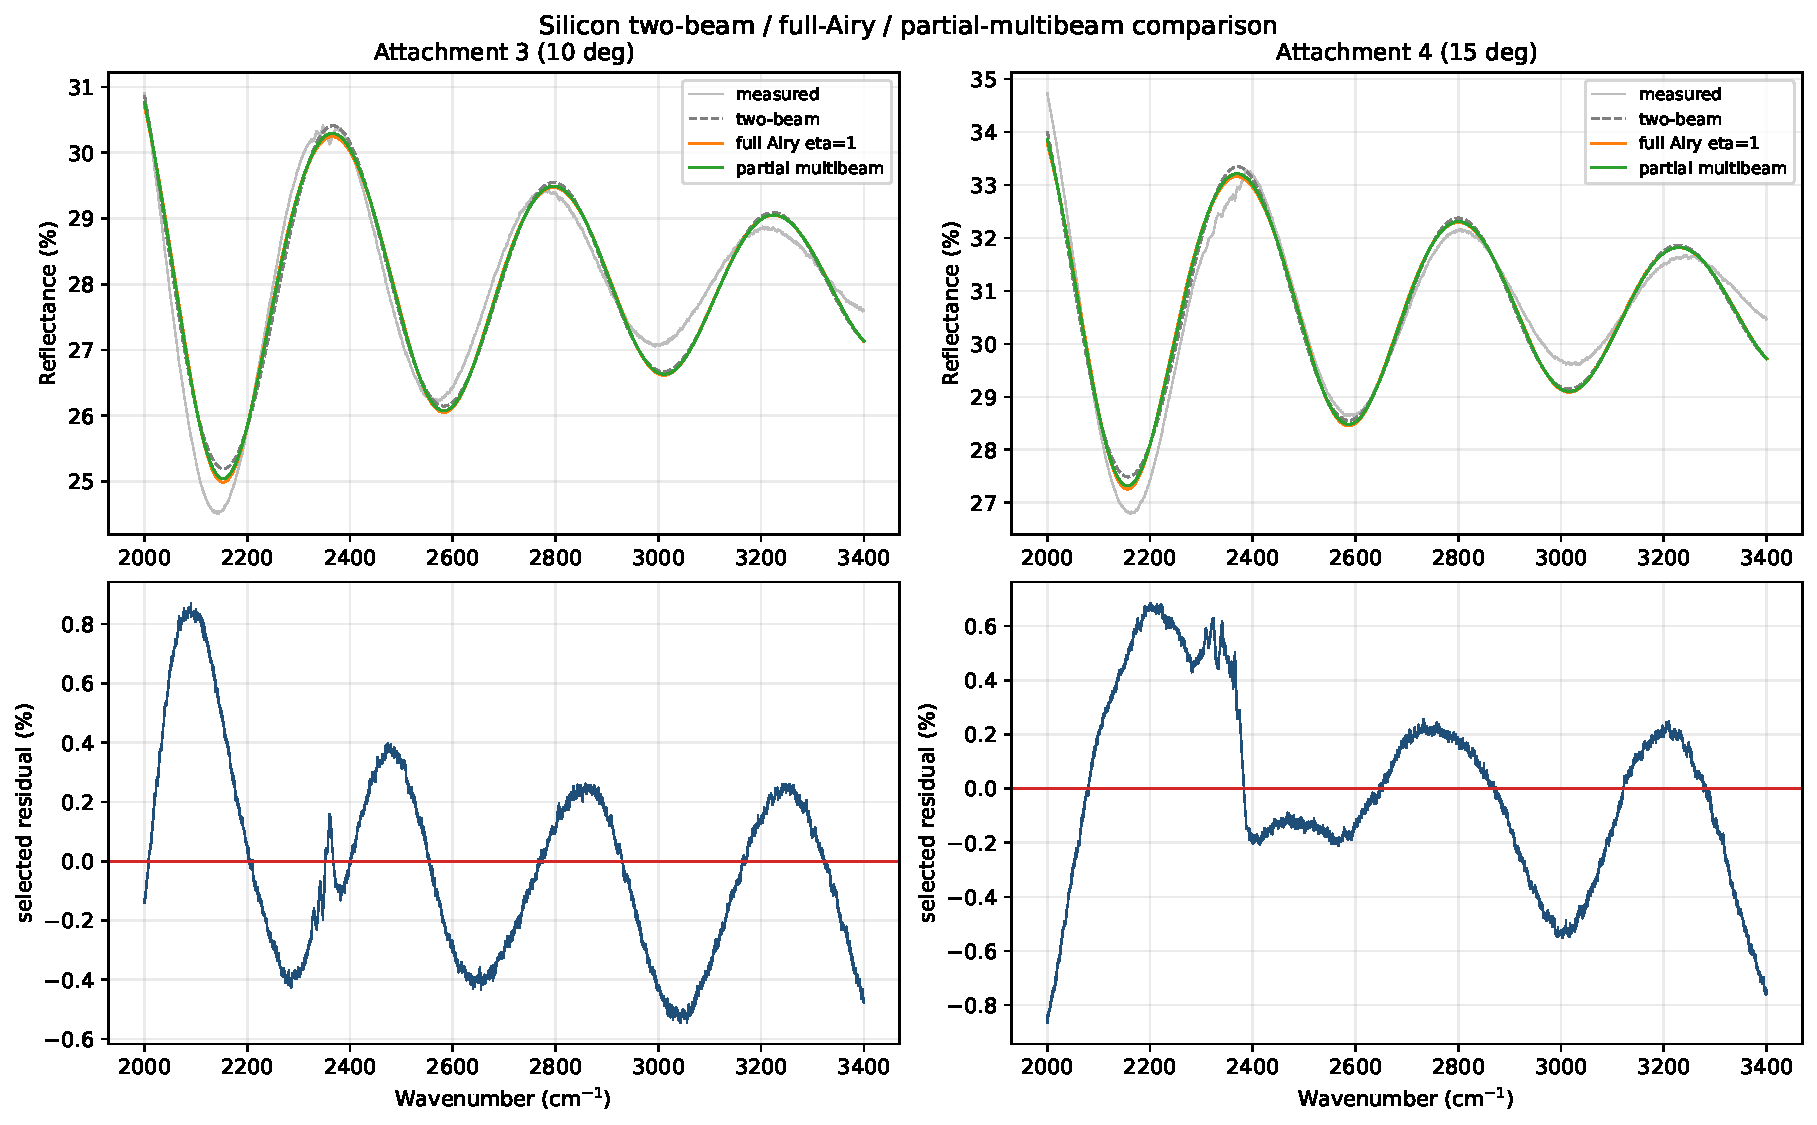
\includegraphics[width=0.96\textwidth]{fig_q3_si_model_comparison.pdf}
  \caption{硅双光束、完全相干 Airy 和部分多光束模型的拟合与残差}
  \label{fig:si-comparison}
\end{figure}

\begin{figure}[H]
  \centering
  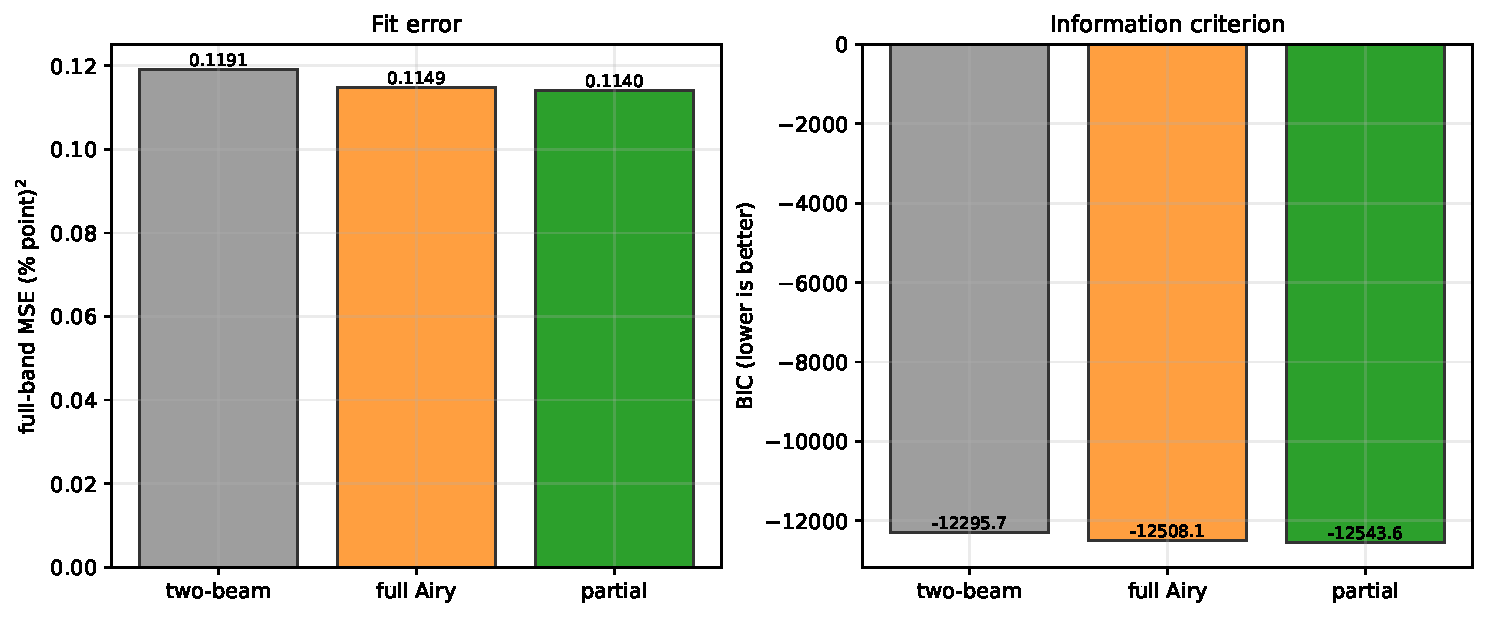
\includegraphics[width=0.96\textwidth]{fig_q3_model_metrics.pdf}
  \caption{三种硅模型在两个入射角下的 RMSE、MAE 和 $R^2$}
  \label{fig:si-metrics}
\end{figure}

\subsection{最终厚度与拟合精度}

选定部分多光束模型的共享厚度和代理参数为
\begin{equation}
  \boxed{d_{\mathrm{Si}}=3.390020843\ \mu\mathrm{m}},\qquad
  \omega_{p,1}=0,\qquad
  \omega_{p,2}=5000\ \mathrm{cm}^{-1},\qquad
  \eta=0.711511282.
  \label{eq:si-final}
\end{equation}
两个代理参数分别落在搜索边界，说明在当前附件和 Sellmeier 假设下它们
存在明显的可辨识性限制；不能把 $0$ 和 $5000$ 当作材料常数的精确测量值。
厚度则由条纹相位在两个角度、全波段上的共同约束给出。

\begin{table}[H]
  \centering
  \caption{硅部分多光束模型的逐角度拟合指标}
  \label{tab:si-metrics}
  \small
  \setlength{\tabcolsep}{5pt}
  \begin{tabular}{cccccc}
    \toprule
    附件 & 角度 & $d(\mu\mathrm{m})$ & $\eta$ & RMSE(\%) & $R^2$\\
    \midrule
    3 & $10^\circ$ & 3.404642207 & 0.705752337 & 0.329699341 & 0.944091273\\
    4 & $15^\circ$ & 3.378301746 & 0.643033365 & 0.345367251 & 0.951433295\\
    \midrule
    联合共享参数 & -- & 3.390020843 & 0.711511282 & -- & --\\
    \bottomrule
  \end{tabular}
\end{table}

联合模型的逐附件指标为：附件 3 的 MAE 为 $0.269305145\%$，绝对残差
95 分位数为 $0.695445153\%$；附件 4 的 MAE 为 $0.281761313\%$，绝对残差
95 分位数为 $0.652598923\%$。逐角度单独拟合的厚度相差
$0.026340461\ \mu\mathrm{m}$，相对于共享厚度约为 $0.777\%$；这项差异
被保留为角度一致性诊断，而不是把两个厚度平均后代替联合反演。

\section{硅结果的可靠性与精度影响}

\subsection{高阶返回强度}

由式 \eqref{eq:rho} 计算得到的 $\rho$ 用于回答“多光束是否足以影响数据”，
而不是作为额外拟合参数。选定部分多光束结果下：

\begin{table}[H]
  \centering
  \caption{硅高阶往返振幅比 $\rho$ 的诊断}
  \label{tab:si-rho}
  \small
  \begin{tabular}{ccccc}
    \toprule
    附件 & 角度 & 中位数 & 95 分位数 & 最大值\\
    \midrule
    3 & $10^\circ$ & 0.047210727 & 0.093441819 & 0.103175524\\
    4 & $15^\circ$ & 0.047209232 & 0.093440754 & 0.103174820\\
    \bottomrule
  \end{tabular}
\end{table}

也就是说，在本模型下，一次额外往返的振幅通常约为 $4.7\%$，高分位数接近
$9.3\%$，不能当成完全可以忽略的微扰。图 \ref{fig:rho} 直观显示了硅和
SiC 的往返强度差异。

\begin{figure}[H]
  \centering
  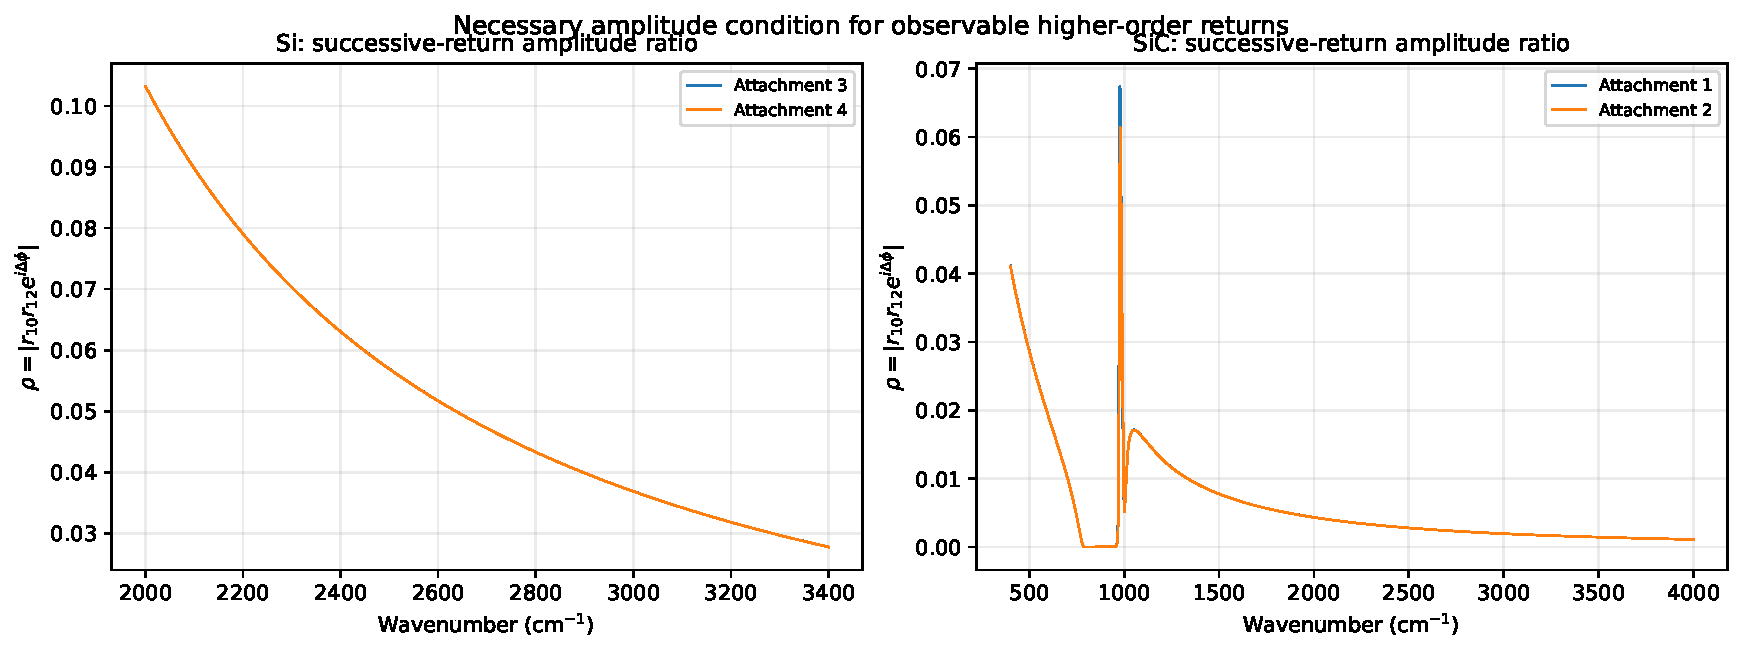
\includegraphics[width=0.96\textwidth]{fig_q3_round_trip_strength.pdf}
  \caption{硅与 SiC 光谱中的高阶往返振幅比 $\rho$}
  \label{fig:rho}
\end{figure}

\subsection{材料代理参数的条件敏感性}

由于硅衬底 Drude 代理参数在主搜索中达到上界，本文分别固定
$\omega_{p,2}=3000,\allowbreak 4000,\allowbreak 5000,\allowbreak 6500,\allowbreak
8000\ \mathrm{cm}^{-1}$，重新优化 $d$、
$\omega_{p,1}$ 和 $\eta$，用于检验厚度是否只是由边界偶然决定。这里把
“重新拟合 MSE 不超过主拟合 1.20 倍”定义为可比较试验；它是透明的诊断阈值，
不是统计置信区间。

\begin{table}[H]
  \centering
  \caption{固定硅衬底代理参数后的条件敏感性}
  \label{tab:sensitivity}
  \small
  \setlength{\tabcolsep}{4pt}
  \begin{tabular}{ccccc}
    \toprule
    固定 $\omega_{p,2}$ & $d(\mu\mathrm{m})$ & $\eta$ & MSE & 相对主拟合\\
    \midrule
    3000 & 3.402324200 & 1.000000 & 0.130720076 & 1.146767\\
    4000 & 3.388881453 & 1.000000 & 0.121972569 & 1.070028\\
    5000 & 3.390020843 & 0.711509 & 0.113990097 & 1.000000\\
    6500 & 3.402834176 & 0 & 2.173655623 & 19.068811\\
    8000 & 2.091392725 & 0.329994 & 36.690471793 & 321.874205\\
    \bottomrule
  \end{tabular}
\end{table}

前三个试验属于可比较集合，厚度范围为
$[3.388881453,3.402324200]\ \mu\mathrm{m}$，跨度
$0.013442747\ \mu\mathrm{m}$，相对主结果的最大偏差约 $0.363\%$。这说明在
当前可接受拟合区域内，厚度对衬底代理参数的条件敏感性小于百分之一；但当
固定值超出数据支持的范围后，MSE 会急剧恶化，此时不能把对应厚度视为有效
备选解。图 \ref{fig:sensitivity} 给出了该诊断的完整结果。

\begin{figure}[H]
  \centering
  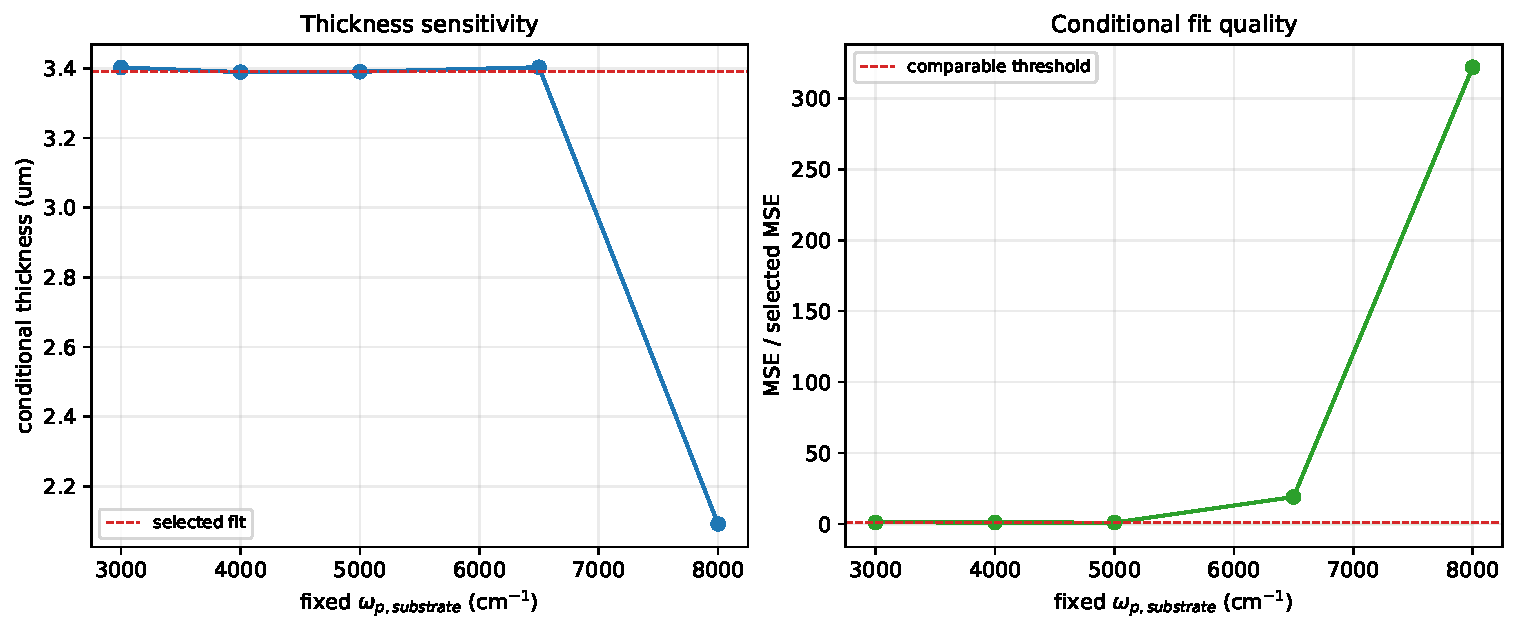
\includegraphics[width=0.96\textwidth]{fig_q3_substrate_sensitivity.pdf}
  \caption{硅衬底 Drude 代理参数的条件敏感性}
  \label{fig:sensitivity}
\end{figure}

\subsection{重复初始化与模型差异}

三个 DE 种子在双光束和完全相干模型上均得到几乎一致的子样本最优值；部分
模型的前两个种子也收敛到同一低 MSE 区域，第三个种子落在明显更差的局部区域，
最终按照完整数据目标函数选择最优候选。这一过程比只报告一次优化结果更能
说明数值求解没有依赖单一随机初始化。

从模型差异看，双光束厚度为 $3.394916326\ \mu\mathrm{m}$，部分多光束厚度
为 $3.390020843\ \mu\mathrm{m}$，修正量为
\begin{equation}
  \Delta d_{\mathrm{Si}}=-0.004895482\ \mu\mathrm{m},
  \qquad \frac{\Delta d}{d_{\mathrm{two-beam}}}\approx-0.1442\%.
  \label{eq:si-correction}
\end{equation}
厚度变化本身不大，但 BIC 和残差结构同时表明多光束模型确实更适合描述
硅光谱；不能只依据厚度数值“看起来接近”就删除多光束项。

\section{附件 1、2 的 SiC 多光束修正}

\subsection{修正策略}

问题三要求若 SiC 也存在多光束，则消除该影响。为保持与问题二的参数定义
一致，代码读取问题二独立目录中的双光束结果作为参考初值，但不直接沿用其
厚度作为最终答案；随后在 $d\in[6.8,8.0]\ \mu\mathrm{m}$ 的邻域内，以
精确相干 Airy 模型 $\eta=1$ 重新优化 SiC 的厚度和六个 Lorentz--Drude
参数。SiC 的背景介电函数写为
\begin{equation}
  \varepsilon_{\mathrm{SiC}}(\sigma)=\varepsilon_\infty
  \frac{\sigma^2-\omega_L^2+i\gamma_L\sigma}
       {\sigma^2-\omega_T^2+i\gamma_T\sigma},
  \label{eq:sic-dielectric}
\end{equation}
其中本次修正采用 $\varepsilon_\infty=6.56$、
$\omega_L=970\ \mathrm{cm}^{-1}$、$\omega_T=798\ \mathrm{cm}^{-1}$，并继续
使用层和衬底各自的 Drude 代理项。用三个确定性的 L-BFGS-B 初始点重复局部
搜索，选择全数据 SSE 最小的结果。

\subsection{修正结果}

问题二双光束参考厚度为
$7.400452153\ \mu\mathrm{m}$。加入精确 Airy 多光束项并重新优化后，得到
\[
\begin{aligned}
  d_{\mathrm{SiC}}^{(3)}&=7.399475918\ \mu\mathrm{m},\\
  \Delta d_{\mathrm{SiC}}&=-0.000976235\ \mu\mathrm{m},\\
  \Delta d/d_{\mathrm{Q2}}&=-0.0131916\%.
\end{aligned}
\]

\begin{table}[H]
  \centering
  \caption{SiC 双光束结果与精确 Airy 修正结果}
  \label{tab:sic-correction}
  \small
  \setlength{\tabcolsep}{3pt}
  \resizebox{\textwidth}{!}{%
  \begin{tabular}{lcccccc}
    \toprule
    模型 & $d(\mu\mathrm{m})$ & $\mathrm{MSE}$ & 附件 1 RMSE(\%)
    & 附件 2 RMSE(\%) & 附件 1 $R^2$ & 附件 2 $R^2$\\
    \midrule
    问题二双光束参考 & 7.400452153 & 0.466583777 & -- & -- & -- & --\\
    问题三精确 Airy & 7.399475918 & 0.455907262 & 0.519276364 & 0.801352970
    & 0.999128235 & 0.998217952\\
    \bottomrule
  \end{tabular}%
  }
\end{table}

精确 Airy 结果下，附件 1 的绝对残差 95 分位数为 $0.756568\%$，附件 2
为 $1.183692\%$。对应的高阶往返振幅比中位数约为 $0.00300$，95 分位数
约为 $0.0226$，明显小于硅的约 $0.0934$。因此 SiC 的高阶返回物理上存在，
但在给定光谱和参数区间中对厚度的影响很弱。图 \ref{fig:sic} 展示了修正前后
模型曲线和残差。

\begin{figure}[H]
  \centering
  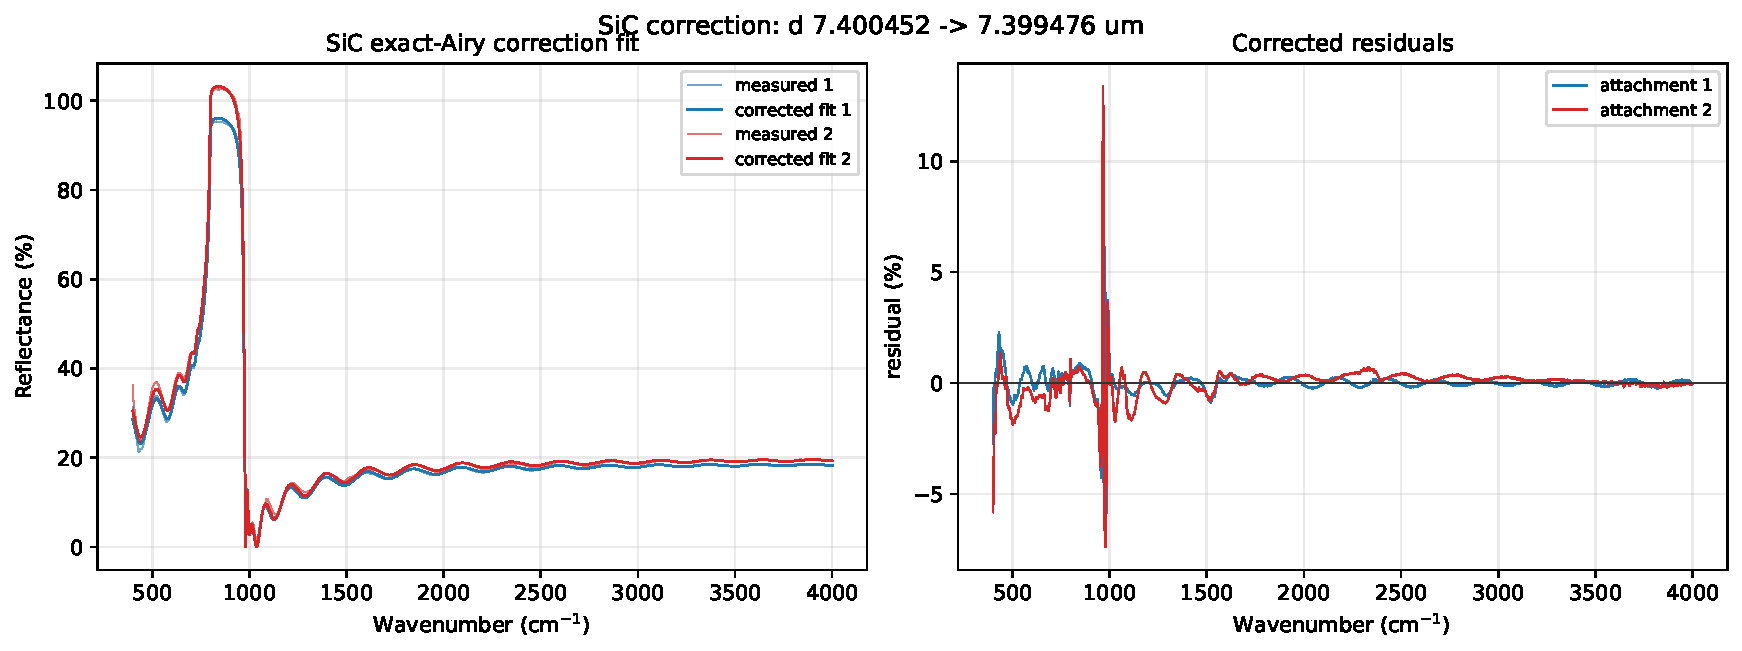
\includegraphics[width=0.96\textwidth]{fig_q3_sic_correction.pdf}
  \caption{SiC 精确 Airy 多光束修正的拟合与残差}
  \label{fig:sic}
\end{figure}

\section{问题三的完整算法流程与复现说明}

完整流程可以概括为图 \ref{fig:workflow}。其中“数据审计”和“结果验证”是
独立于优化器的步骤，用于防止把输入异常、材料假设或局部最优误认为多光束
结论。

\begin{figure}[H]
  \centering
  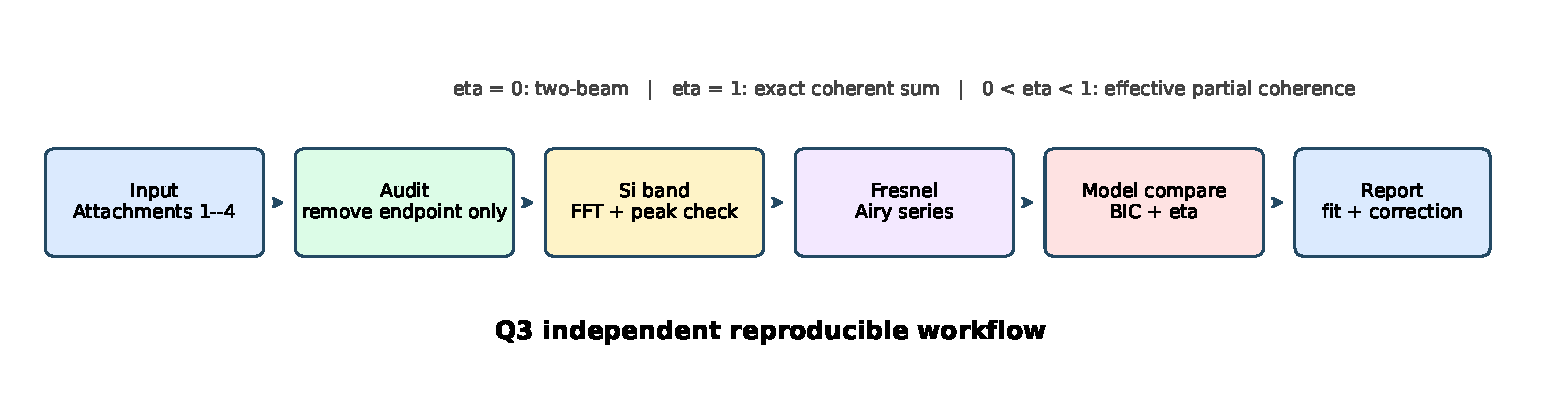
\includegraphics[width=0.96\textwidth]{fig_q3_workflow.pdf}
  \caption{问题三从输入审计到结果验收的算法流程}
  \label{fig:workflow}
\end{figure}

交付目录结构为：
\begin{verbatim}
F:/数学建模/2025B/题目3_完整交付/
  code/solve_q3.py                 主求解、审计、拟合和结果导出
  code/make_q3_figures.py          根据已保存结果生成全部论文图
  data/附件1.xlsx ... 附件4.xlsx   原始附件副本（只读）
  data/B题.pdf                     题面副本
  data/processed/                  仅删除首个 0% 端点后的审计 CSV
  results/q3_result.json           主结果、参数、指标和优化记录
  results/q3_substrate_sensitivity.json
  results/q3_si_predictions.csv
  results/q3_sic_correction_predictions.csv
  results/data_audit.json
  figures/                          每幅图的 PDF、PNG 和 manifest
  paper/q3_solution.tex             本文 LaTeX 源文件
  paper/build/q3_solution.pdf      编译后的本文
\end{verbatim}

在 Windows PowerShell 中可按下面顺序复现：
\begin{verbatim}
cd F:/数学建模/2025B/题目3_完整交付
python code/solve_q3.py
python code/make_q3_figures.py
cd paper
xelatex -halt-on-error -output-directory=build `
  q3_solution.tex
xelatex -halt-on-error -output-directory=build `
  q3_solution.tex
\end{verbatim}

求解脚本会重新读取附件并覆盖本独立目录中的派生结果，但不会修改原始 Excel；
绘图脚本只读取 JSON 和预测 CSV，不重新优化。所有表格中的数值均来自本目录
的 JSON/CSV，而不是手工抄录的中间屏幕输出。

\section{结论与局限性}

\begin{enumerate}[label=结论\arabic*：,leftmargin=5em]
  \item 多光束干涉需要相干性、高阶返回非零且足够强、相位可分辨以及空间/角度
  平均不完全洗掉条纹。$\rho$ 是返回强度是否可能被观测到的直接诊断，但不是
  单独的充分条件。
  \item 附件 3、4 的硅光谱在 $2000\sim3400\ \mathrm{cm}^{-1}$ 共同区间内，
  部分多光束模型相对双光束的 BIC 改善为 $247.882121$，拟合
  $\eta=0.711511282$，因此判定存在可观测多光束效应。最终厚度为
  $3.390020843\ \mu\mathrm{m}$。
  \item 若只用双光束，硅厚度为 $3.394916326\ \mu\mathrm{m}$，与多光束结果
  相差约 $0.1442\%$；数值差异不大，但模型选择和残差结构不能忽略。
  \item SiC 附件 1、2 用精确 Airy 模型修正后的厚度为
  $7.399475918\ \mu\mathrm{m}$，相对问题二双光束结果变化约 $-0.0132\%$，
  所以其多光束修正对最终厚度很小。
\end{enumerate}

本结果有四点边界需要明确：第一，硅 Sellmeier 系数和 Drude 代理是因为附件
没有提供逐点复折射率而作出的条件性假设；第二，两个角度的 affine 校准提高了
对仪器幅值误差的鲁棒性，但也增加了模型自由度；第三，硅衬底代理参数达到
搜索上界，表明材料参数本身不可完全由当前数据识别，文中的敏感性分析只证明
在可接受拟合区间内厚度较稳定；第四，Differential Evolution 加 L-BFGS-B
给出的是经过多种种子检验的高质量数值解，而不是数学意义上的全局最优证明。
因此，本文的厚度结论应理解为“在所列光学假设、波段和校准模型下的可复现
反演结果”。

\end{document}
